\documentclass[a4paper,11pt]{article}

% --- Packages ---
\usepackage[utf8]{inputenc}
\usepackage[T1]{fontenc}
\usepackage{geometry}
\usepackage{graphicx}
\usepackage{svg}
\usepackage{booktabs}
\usepackage{tabularx}
\usepackage{siunitx}
\usepackage{amsmath}
\usepackage{amssymb}
\usepackage{hyperref}
\usepackage{caption}
\usepackage{fancyhdr}
\usepackage{subcaption}
\usepackage{float}
\usepackage[style=ieee, backend=biber]{biblatex}

% --- Configuration ---
\geometry{top=2.5cm, bottom=2.5cm, left=2.5cm, right=2.5cm}

\addbibresource{references.bib}

\sisetup{
    output-decimal-marker = {.},
    group-digits = true,
    per-mode = symbol
}

% SVG Settings
% DO NOT use \svgsetup{convert=true} with the standard 'svg' package.
% Just ensure Inkscape is in PATH and compile with --shell-escape.
% The 'svg' package will automatically call Inkscape to convert .svg to .pdf.

\hypersetup{
    colorlinks=true,
    linkcolor=blue,
    filecolor=magenta,      
    urlcolor=cyan,
    pdftitle={HumanEd: Oar Robot Proposal},
    pdfauthor={Benjamin McEwan}
}

% --- DOCUMENT -------------------------------------------------------------------------------------
\begin{document}

\title{\textbf{HumanEd: "Oar" Robot}}
\author{Benjamin McEwan}
\date{\today}
\maketitle

\tableofcontents


% --- Overview -------------------------------------------------------------------------------------
\newpage
\section{Overview}\label{sec:overview}
\begin{figure}[h!]
    \centering
    % NO 'crop' option here. Just the filename.
    % Ensure you cropped the SVG in Inkscape first!
    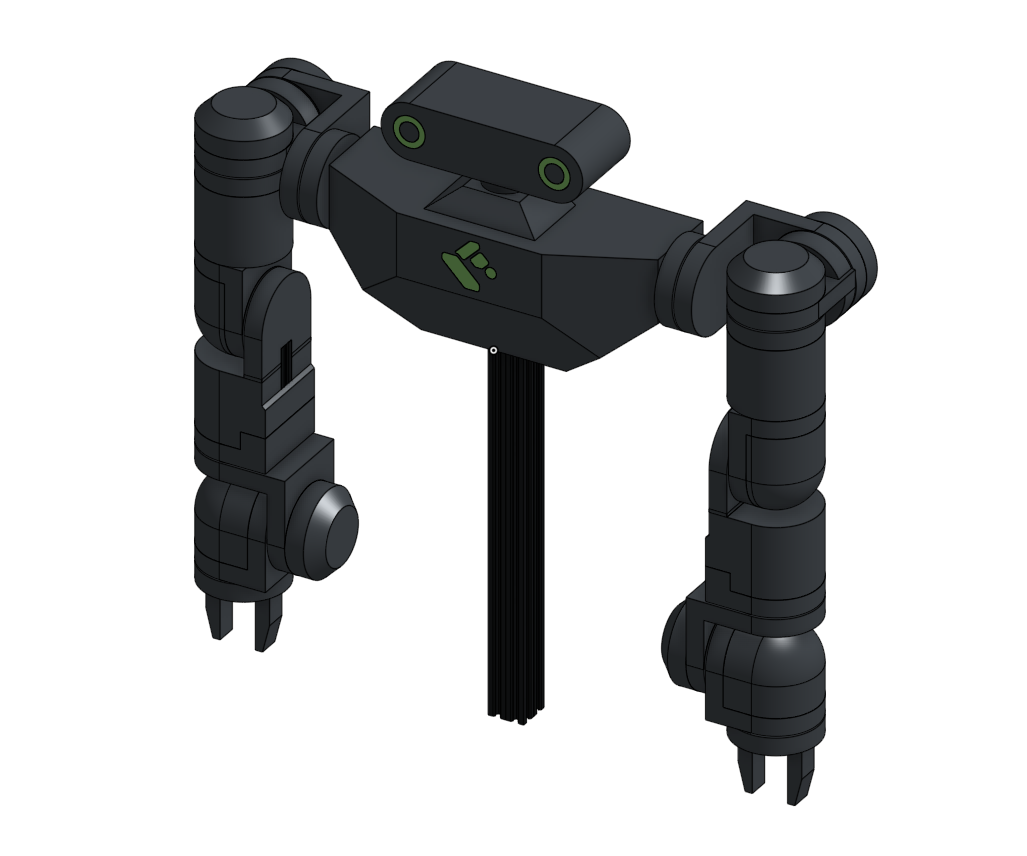
\includegraphics[width=0.5\linewidth]{img/mockup_shell.png} 
    \caption{Mockup of Oar}
    \label{fig:mockup}
\end{figure}

The "Oar" robot is a humanoid robot comprised of a rigidly-supported torso, a head placed upon an actuated neck, and two 7 degree of freedom robotic arms. A basic mockup of Oar is shown in Figure \ref{fig:mockup}.

The design goals for Oar are as follows:
\begin{itemize}
    \item Demonstrate the strengths, capabilities, and pitfalls of 3D printed actuator gearhead designs and serve as a design study that may inform future HumanEd humanoid robots.
    \item Provide a reliable humanoid arm system capable of accurately positioning the end-effector for experimental and demonstratory purposes. Experimental usages includes testing of end-effector designs (grippers, hands), a real-world interface for computer vision experiments, and a follower-arm for teleoperations experiments. Demonstrations may include various tasks that could be performed at fairs or open days at which the society of HumanEd may be present.
    \item Provide a reasonable suite of sensors that can be interfaced with for experiments. Such experiments may include computer vision or reinforcement learning projects.
\end{itemize}

This proposal will focus primarily on the development of the robot's arms as they are considered to be the primary engineering challenge, however some notes on the body, neck/head, and end-effector will still be made.

\subsection{A note on the name}
The name "Oar" has been derived from the first line of the poem "Basking Shark" by Scottish poet Norman MacCaig, which reads:

\begin{center}
    \textit{To stub an \textbf{oar} on a rock where none should be}
\end{center}

The poem is a discussion on themes of the origins of life and the place of humanity in the timeline of evolution. The decision to choose this poem to name the robot reflects the robot's intended position as HumanEd's first full-scale humanoid robot. It is also intended for an inscription of the poem to be placed somewhere on the robot in commemoration of this poem.


% --- ARM STRUCTURE --------------------------------------------------------------------------------
\newpage
\section{Arm Design}\label{sec:arm_design}
\begin{figure}[htbp]
    \centering
    \begin{subfigure}[b]{0.38\textwidth}
      \centering
      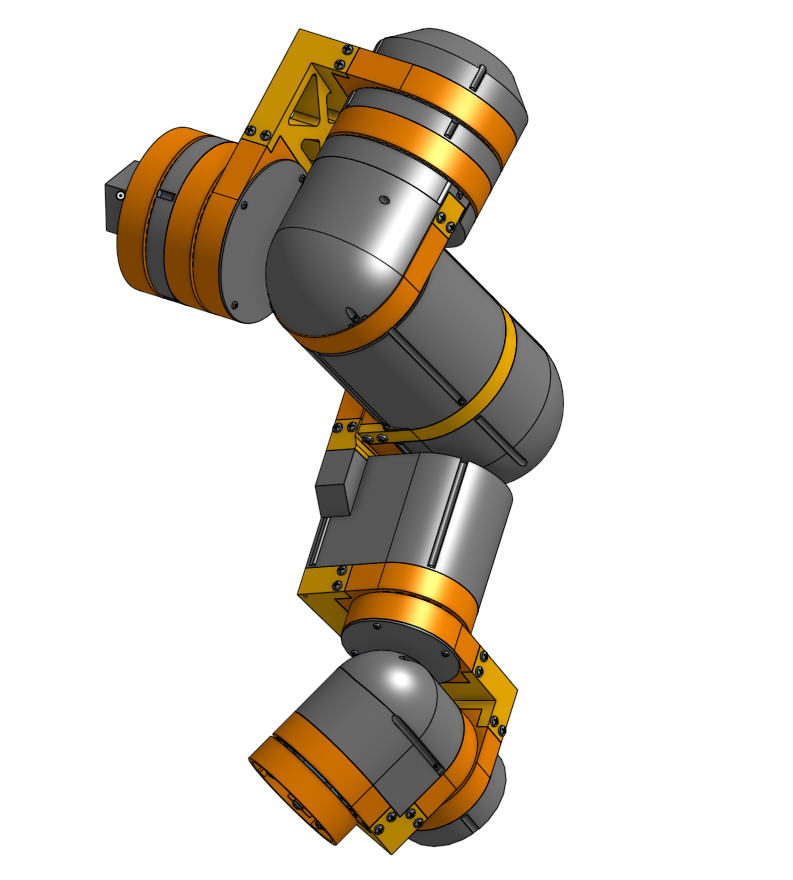
\includegraphics[width=\textwidth]{img/arm_posed.png}
      \caption{Arm in a posed position to demonstrate the joints.}
      \label{fig:arm_posed}
    \end{subfigure}
    \hfill
    \begin{subfigure}[b]{0.3\textwidth}
      \centering
      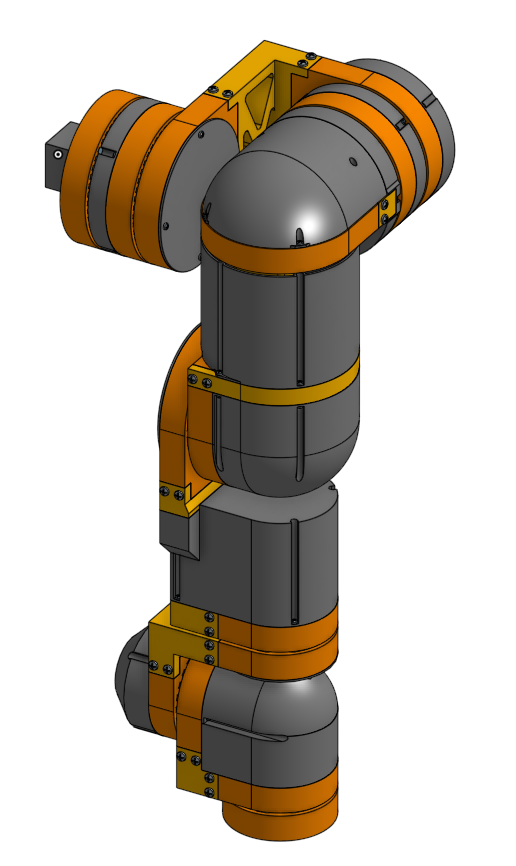
\includegraphics[width=\textwidth]{img/arm_rest_shell.png}
      \caption{Arm at rest with aesthetic shells.}
      \label{fig:arm_rest_shell}
    \end{subfigure}
    \hfill
    \begin{subfigure}[b]{0.3\textwidth}
      \centering
      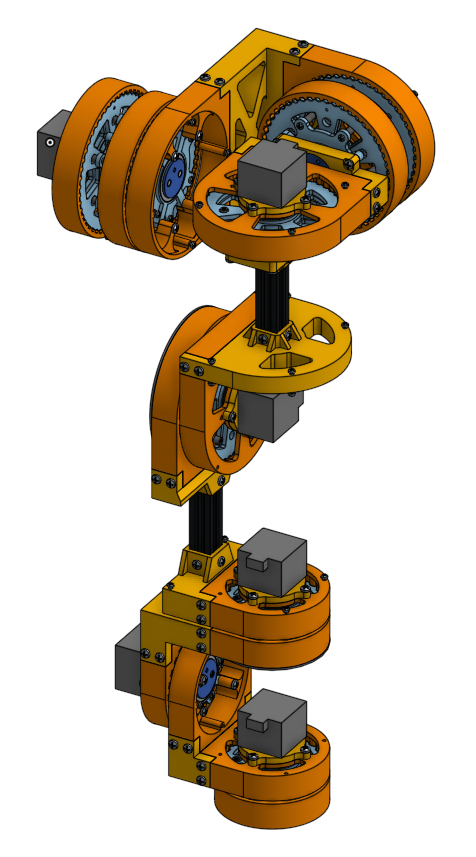
\includegraphics[width=\textwidth]{img/arm_rest_noshell.png}
      \caption{Arm at rest without aesthetic shells.}
      \label{fig:arm_rest_noshell}
    \end{subfigure}
  
    \caption{The preliminary arm design for Oar (left arm).}
    \label{fig:arms}
\end{figure}


Figure \ref{fig:arm_posed} shows the complete preliminary arm design in a posed state, with Figure \ref{fig:arm_rest_shell} in the resting positon. The parts coloured in dark gray (excluding motors) are aesthetic "shells", which have been hidden in Figure \ref{fig:arm_rest_noshell}. It should be noted that the primary focus of this preliminary design the general structure of the arm and the design of the actuator gearheads; the aesthetic shells have been very roughly constructed for visual purposes and are missing key features such as cutouts for cable management.

The design is comprised of primarily 3D printed parts, and two pieces of $20\,\si{mm} \times 20\,\si{mm}$ aluminium extrusion. The motors used in the preliminary design are 17HS3401S stepper motors, however these are not critical to the design as the mounting holes can be easily adjusted. One option may be to swap out these motors for a lighter model, provided that the produced torque is comparable, as the current motors contribute a significant amount of mass at $220\,\si{g}$ each.

The arm is roughly $600\,\si{mm}$ in length. Most of the length comes from the large size of the actuators, however about $200\,\si{mm}$ is contributed by the Aluminium extrusion. The extrusion was added for two reaons: (i) to increase the reach of the arm and bring it in-line with the goal of being a "full-scale" humanoid arm; (ii) to support the arm links at points of high bending moments. The primary downside of this length is that it decreases the potential maximum payload of the arm. This drawback has been overruled in favour of greater reach in the preliminary design as arm dexterity and "human-ness" are seen as more significant goals for the project than maximum payload, if however, maximum payload becomes an important goal, then the inclusion of the extruded bars may be reconsidered and actuators instead mounted end-to-end to one another.

Each of the 3D printed parts (excluding the aesthetic shells) has been designed to require minimal to no support structures during printing and to feature various weight saving cutouts where possible. The parts will be prototyped using PLA, with the final designs printed in PETG.

\begin{table}[h!]
    \centering
    
    \begin{tabular}{|c|c|}
        \hline
        Joint & Gearhead Ratio \\
        \hline
        Shoulder Pitch & 96:1 (Comprised of two 48:1 gearheads in series) \\
        Shoulder Roll & 96:1 (Comprised of two 48:1 gearheads in series) \\
        Shoulder Yaw & 48:1 \\
        Elbow & 48:1 \\
        Wrist Roll 1 & 24:1 \\
        Wrist Pitch & 24:1 \\
        Wrist Roll 2 & 24:1 \\
        \hline
       \end{tabular}

    \caption{Gear ratios present at each joint.}
    \label{tab:joints}
\end{table}

The arm follows the common humanoid arm model of a 3-DOF shoulder and a 3-DOF wrist connected by a 1-DOF elbow. A joint diagram can be seen in \S~\ref{sec:forward_kinematics}. Table \ref{tab:joints} shows the gear ratios of each joint's gearheads. The ratios have been chosen such that each joint can produce its required output torques while also comprising of only two primary gearhead designs. The gearheads are of a cycloidal design, as detailled in \S~\ref{sec:gearheads}.

The following sections detail the analyses from which this arm design has been developed.

\subsection{Forward Kinematics \& Preliminary Torque Analysis}\label{sec:forward_kinematics}
\begin{figure}[h!]
    \centering
    % NO 'crop' option here. Just the filename.
    % Ensure you cropped the SVG in Inkscape first!
    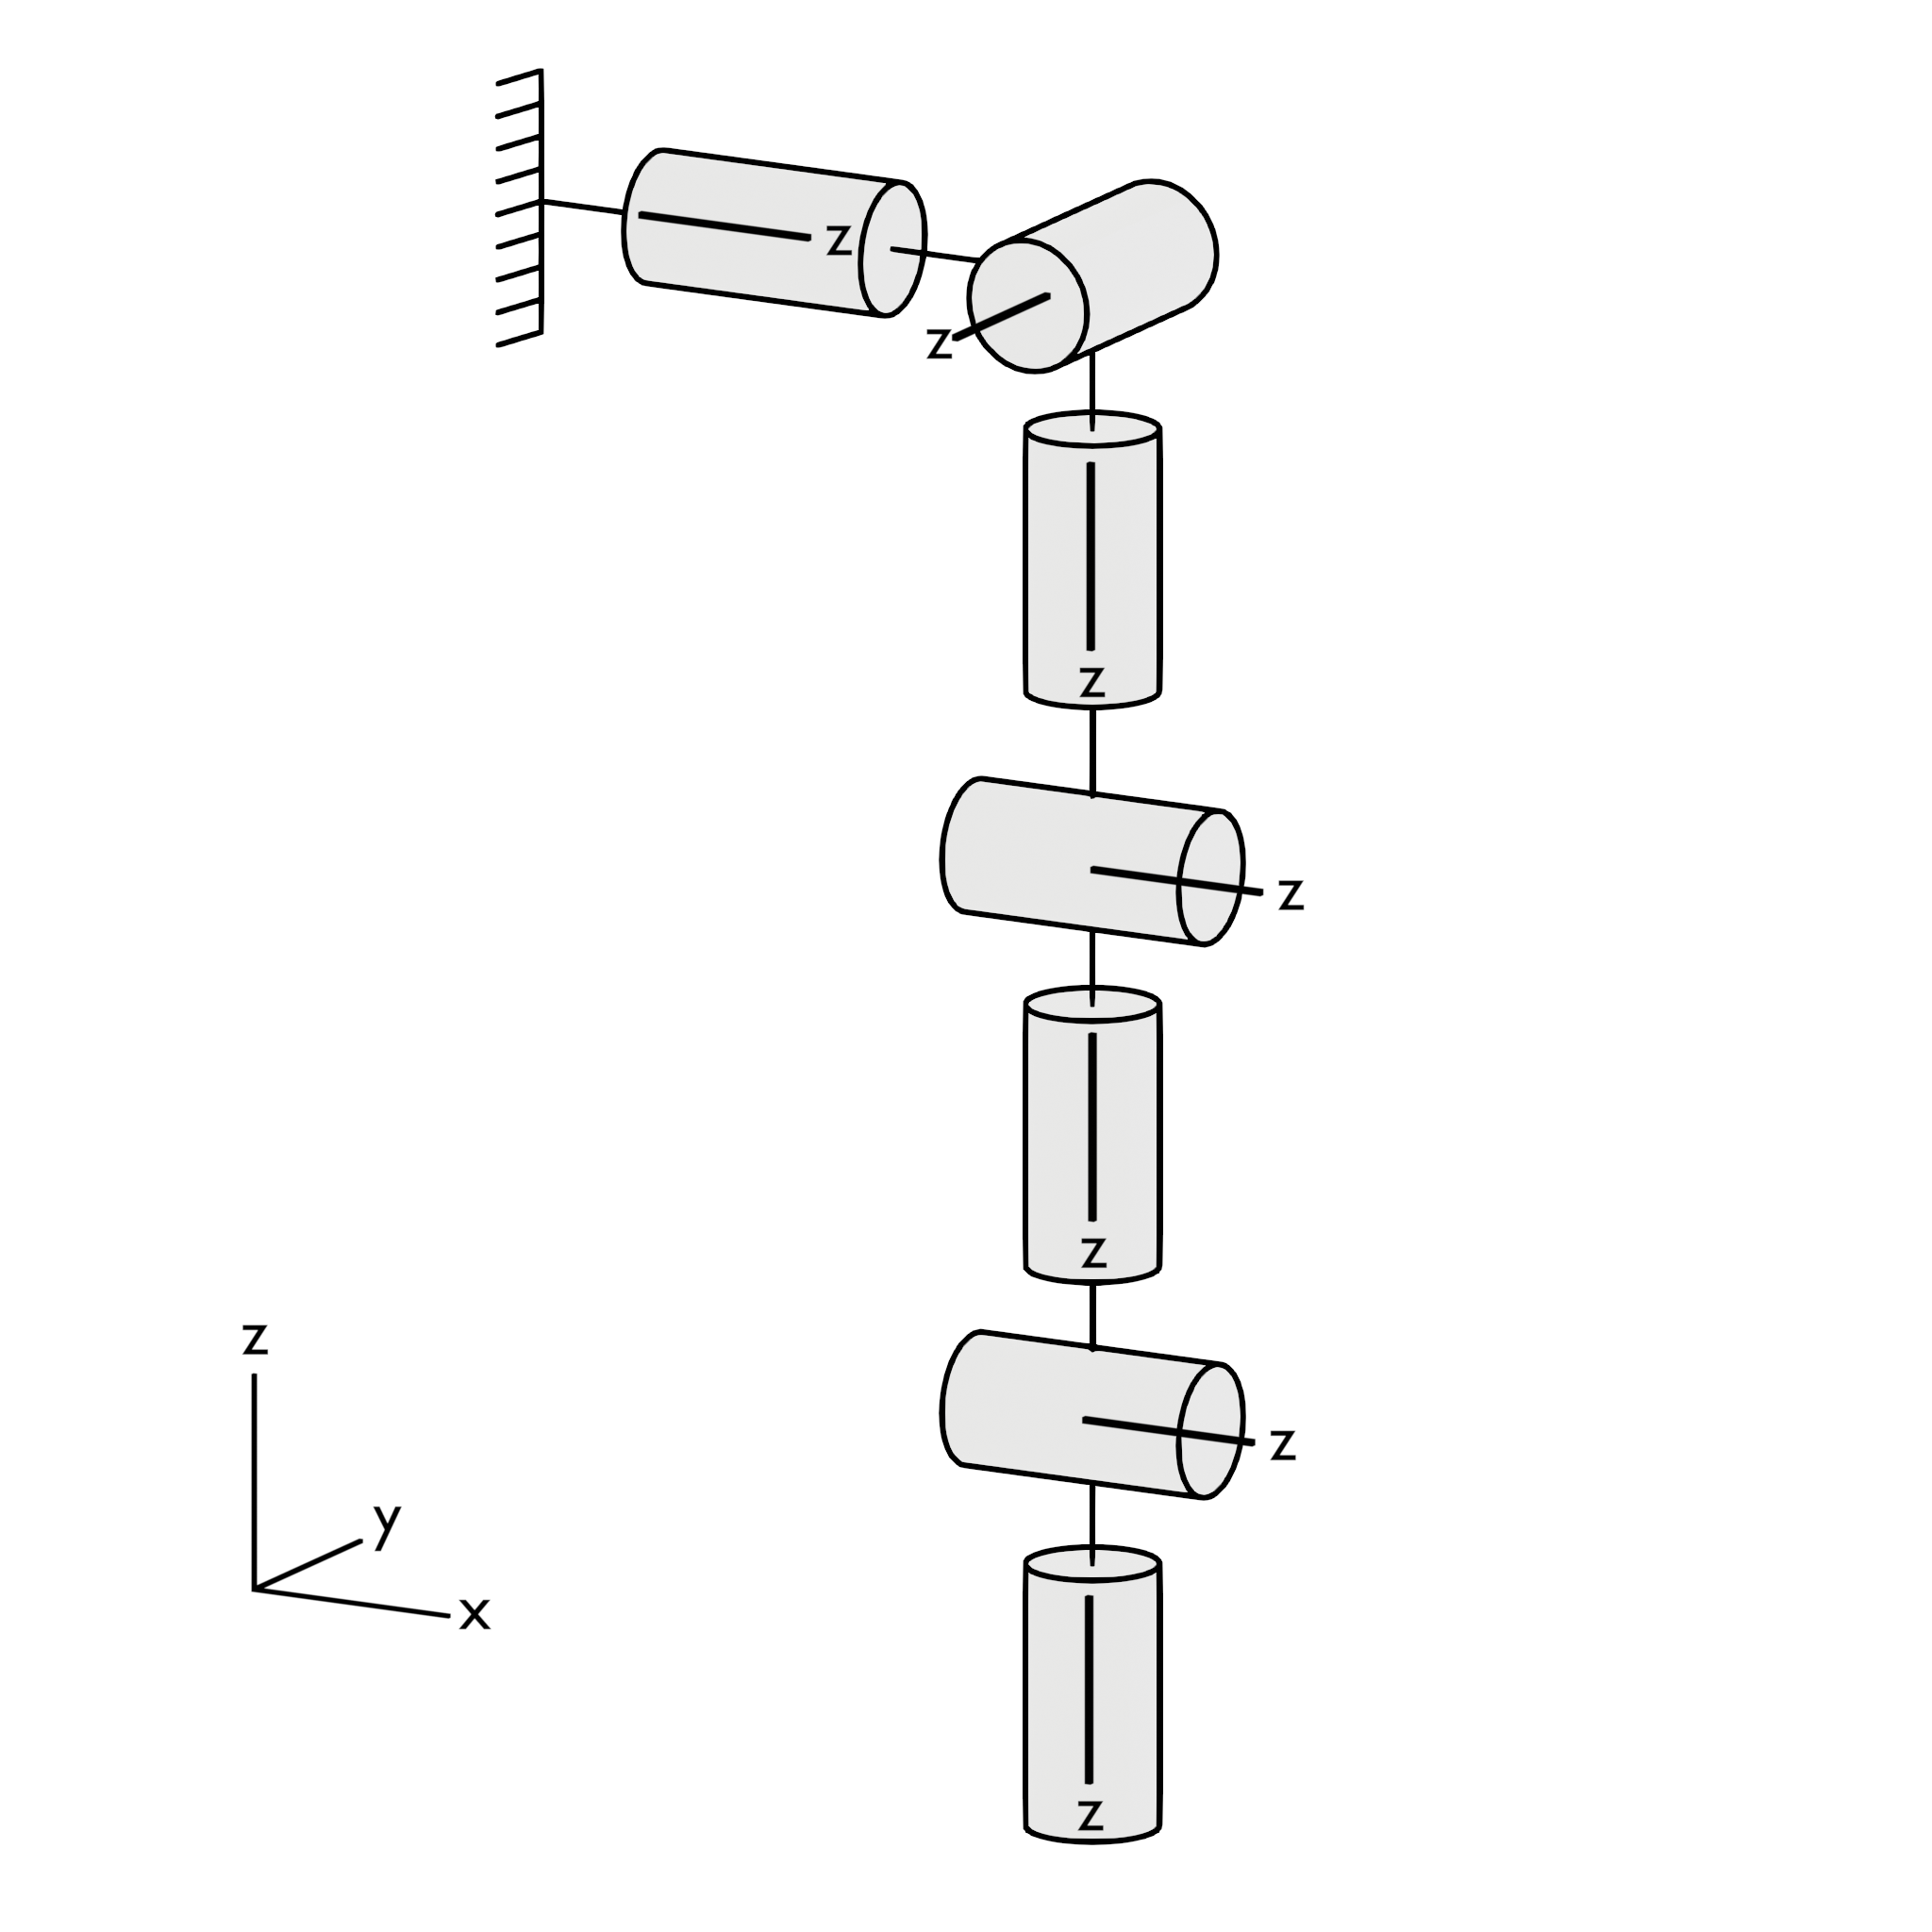
\includegraphics[width=0.6\linewidth]{img/joint_diagram.png} 
    \caption{Joint diagram of Oar's left arm}
    \label{fig:joints}
\end{figure}

Figure \ref{fig:joints} shows the joint diagram of Oar's left arm. All of the joints shown are revolute joints. For the purpose of the forward kinematics analysis, all three of the shoulder joints will be considered coincident, and all three of the wrist joints will also be considered coincident. The vertical distance between the shoulder jonts and the elbow joint is taken as $L_1$, and the distance between the elbow joint and the wrist joints as $L_2$.

The resting position of the end-effector frame $\{\mathrm{b}\}$ is a right-handed set of axes rotated by $pi$ radians about the $\mathrm{x}$-axis such that the $\mathrm{z}_{b}$ axis points downwards.

The forward kinematics of the arm can then be defined via the method as described by \textcite[\S~4.1]{modernrobotics}. $\theta \in \mathbb{R}^{7}$ is the vector of all joint positions of the arm, and $M \in SE(3)$ is the transformation matrix of the end-effector when the arm is in its resting position, defined as
\begin{equation*}
    \quad M = \begin{bmatrix} 
        1 & 0 & 0 & 0 \\ 
        0 & -1 & 0 & 0 \\ 
        0 & 0 & -1 & -(L_{1}+L_{2}) \\
        0 & 0 & 0 & 1 
    \end{bmatrix} \in SE(3)
\end{equation*}
The screw axes $\mathcal{S}_{i}$, $i=1,\dots,7$, represented in the space frame, can be seen as:
\begin{equation*}
    \mathcal{S}_{1} = \begin{bmatrix}
        1 \\ 0 \\ 0 \\ 
        0 \\ 0 \\ 0
    \end{bmatrix}
    ,\quad
    \mathcal{S}_{2} = \begin{bmatrix}
        0 \\ -1 \\ 0 \\ 
        0 \\ 0 \\ 0
    \end{bmatrix}
    ,\quad
    \mathcal{S}_{3} = \begin{bmatrix}
        0 \\ 0 \\ -1 \\ 
        0 \\ 0 \\ 0
    \end{bmatrix}
    ,\quad
    \mathcal{S}_{4} = \begin{bmatrix}
        1 \\ 0 \\ 0 \\ 
        0 \\ -L_{1} \\ 0
    \end{bmatrix}
\end{equation*}

\begin{equation*}
    \mathcal{S}_{5} = \begin{bmatrix}
        0 \\ 0 \\ -1 \\ 
        0 \\ -(L_{1}+L_{2}) \\ 0
    \end{bmatrix}
    ,\quad
    \mathcal{S}_{6} = \begin{bmatrix}
        1 \\ 0 \\ 0 \\ 
        0 \\ -(L_{1}+L_{2}) \\ 0
    \end{bmatrix}
    ,\quad
    \mathcal{S}_{7} = \begin{bmatrix}
        0 \\ 0 \\ -1 \\ 
        0 \\ -(L_{1}+L_{2}) \\ 0
    \end{bmatrix}
\end{equation*}

Which yields the forward kinematics equation where $T(\theta) \in SE(3)$ is the transformation matrix describing the position and orientation of the end-effector given the joint positions $\theta$:

\begin{equation}\label{eq:fk}
    T(\theta) = 
    e^{\displaystyle [\mathcal{S}_{1}]\theta_{1}}
    e^{\displaystyle [\mathcal{S}_{2}]\theta_{2}}
    e^{\displaystyle [\mathcal{S}_{3}]\theta_{3}}
    e^{\displaystyle [\mathcal{S}_{4}]\theta_{4}}
    e^{\displaystyle [\mathcal{S}_{5}]\theta_{5}}
    e^{\displaystyle [\mathcal{S}_{6}]\theta_{6}}
    e^{\displaystyle [\mathcal{S}_{7}]\theta_{7}}
    M
\end{equation}

Equation \ref{eq:fk} can then be used to find the space Jacobian $J_{s}(\theta) \in \mathbb{R}^{6 \times 6}$ of the arm's end-effector via the expression:
\begin{equation}\label{eq:jacobian}
    J_{si}(\theta) = 
    \left[\mathrm{Ad}_{\displaystyle e^{\displaystyle [S_{1}]\theta_{1}}\cdots e^{\displaystyle [S_{i-1}]\theta_{i-1}}e^{\displaystyle [S_{i}]\theta_{i}}}\right]
    \mathcal{S}_{i}
\end{equation}
where $J_{si}(\theta)$ is the $i$th columns of $J_s(\theta)$. This can then be used to perform a statics analysis of the arm via the equation
\begin{equation}\label{eq:statics}
    \tau = J_{s}^{T}(\theta)\mathcal{F}_{s}
\end{equation}
where $\mathcal{F}_{s}$ is a wrench applied to the end-effector, and $\tau$ is the resulting vector of torques required in each joint to resist $\mathcal{F}_{s}$.

The method for performing this analysis is detailed in \cite[\S~5]{modernrobotics} and for this robot results in matrices that are too large and complex to be reasonably computed by hand for every possible configuration of interest. As such Equations, \ref{eq:fk}, \ref{eq:jacobian}, and \ref{eq:statics} were implemented into a python script to complete the analysis.

Using the python script, a variety of configurations were tested for a $600\,\si{g}$ payload. This is greater than the reasonable payload considered as a goal for the final arm design (which sits at $300\,\si{g}$ to $500\,\si{g}$), however performing early computations for an oversized payload was done as the robot must have a factor of safety on top of its specified capabilties. An additional reason is that this analysis does not take into account the masses of the links themselves.

The tested configurations showed that the maximum torque required of the arm's joints would take place in the shoulder pitch, shoulder roll, and elbow, and would be roughly of a magnitude of $4\,\si{N m}$. Considering this figure, and the estimated efficiency of a 3D printed cycloidal gearhead of 40\%-60\%, the primary gearhead ratio of 48:1 was chosen.

Following this, a series of prototype were developed in order to inform the rest of the preliminary arm design. These are detailed in \S~\ref{sec:gearheads},.

\subsection{Gearhead Efficiency Requirement Analysis}

% --- GEARHEADS ------------------------------------------------------------------------------------
\newpage
\section{Gearhead Design}\label{sec:gearheads}

Cycloidal drives have been chosen for the actuators of the arm. This is primarily due to their affinity for being produced using FDM printing when compared to planetary or strain-wave gear systems, wherein the former presents difficult to achieve tolerances (as well as comparatively low reduction ratios) and the latter requires the development of a flexible element.

The following sections detail the development of a prototype gearhead. The model of stepper motor used was the 17HS3401S, which was ran at a speed of $100\,\si{RPM}$ and measured to have a dynamic torque of $0.17\,\si{N m}$\footnote{Used to drive a rudimentary pulley of diameter $30\,\si{mm}$ and found to be capable of lifting a maximum of $575\,\si{g}$.}.

The output torque produced by each prototype gearhead was tested using various masses suspended from a $30\,\si{cm}$ bar of $20\,\si{mm} \times 40\,\si{mm}$ aluminium extrusion attached from the centerpoint of the gearhead's output.

\subsection{First Prototype - 24:1}\label{sec:proto1}

\begin{figure}[htbp]
    \centering
    \begin{subfigure}[b]{0.45\textwidth}
      \centering
      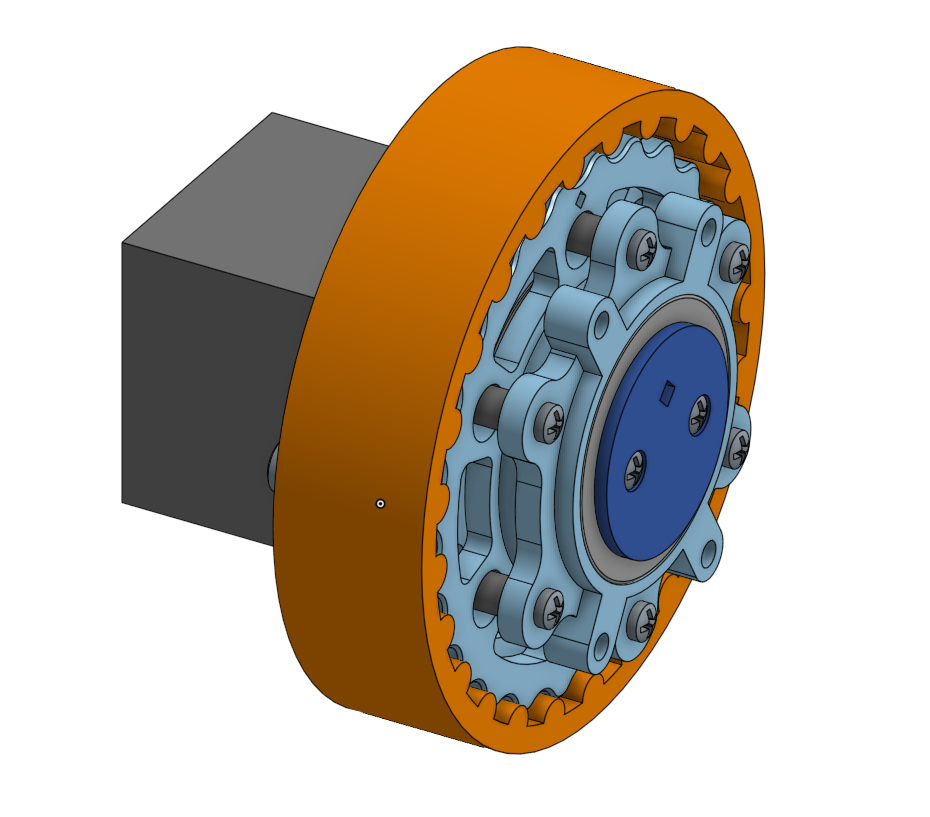
\includegraphics[width=\textwidth]{img/proto1_a.png}
      \caption{Isometric view.}
      \label{fig:proto1a}
    \end{subfigure}
    \hfill
    \begin{subfigure}[b]{0.45\textwidth}
      \centering
      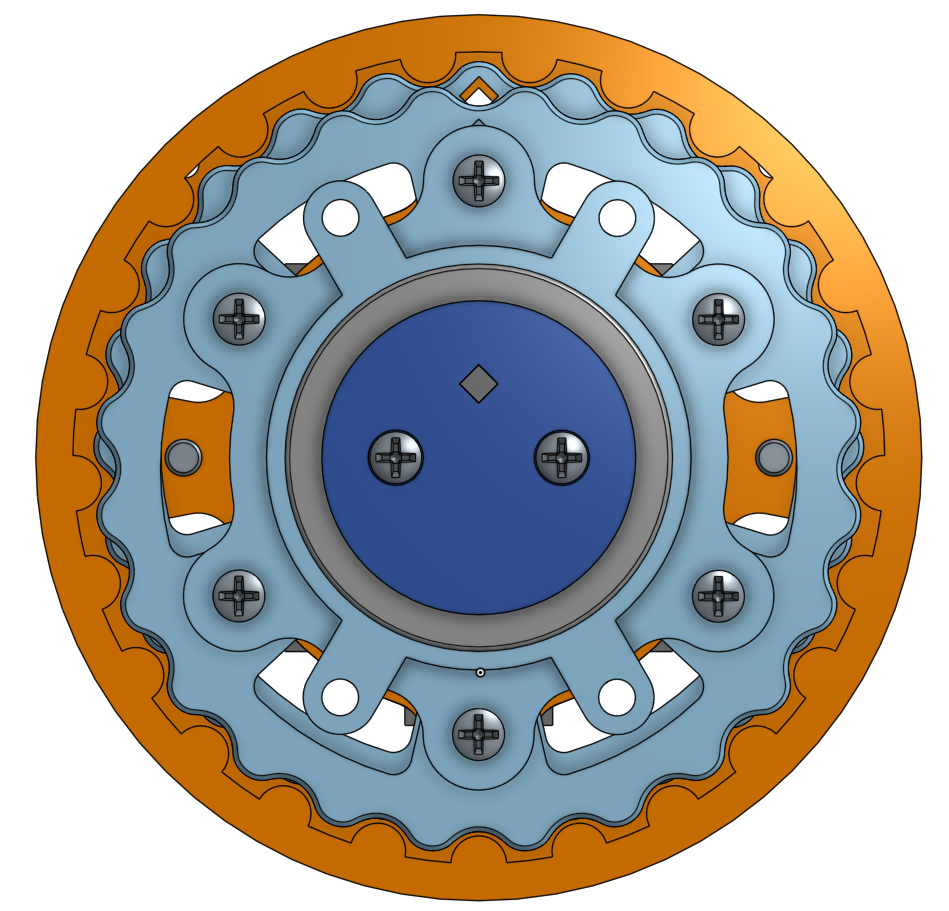
\includegraphics[width=\textwidth]{img/proto1_b.png}
      \caption{View of disc plane.}
      \label{fig:proto1b}
    \end{subfigure}
  
    \caption{The prototype 24:1 gearhead design.}
    \label{fig:proto1}
\end{figure}

Figure \ref{fig:proto1} shows the design of the first prototype gearhead that was built and tested. This prototype was built with a 24:1 reduction ratio, half of the primary 48:1 reduction ratio calculated in \S~\ref{sec:forward_kinematics}. Figure \ref{fig:proto1a} shows an isometric view of the design with all housings included, Figure \ref{fig:proto1b} shows a view from the plane of the gearhead's cycloidal discs, with the output housing hidden for clarity.

The design is almost entirely comprised of FDM printed parts, with the only exceptions being the bearings, screws, and of course stepper motor.

The gearhead was seen to be able to achieve a maximum output torque of roughly $1.0\,\si{N m}$, which gives an efficiency of about 25\%. This is, needless to say, a poor result, however it did show that the design was able to successfully increase the output torque of the motor.

\subsection{Second Prototype - 48:1}\label{sec:proto2}

\begin{figure}[h!]
    \centering
    % NO 'crop' option here. Just the filename.
    % Ensure you cropped the SVG in Inkscape first!
    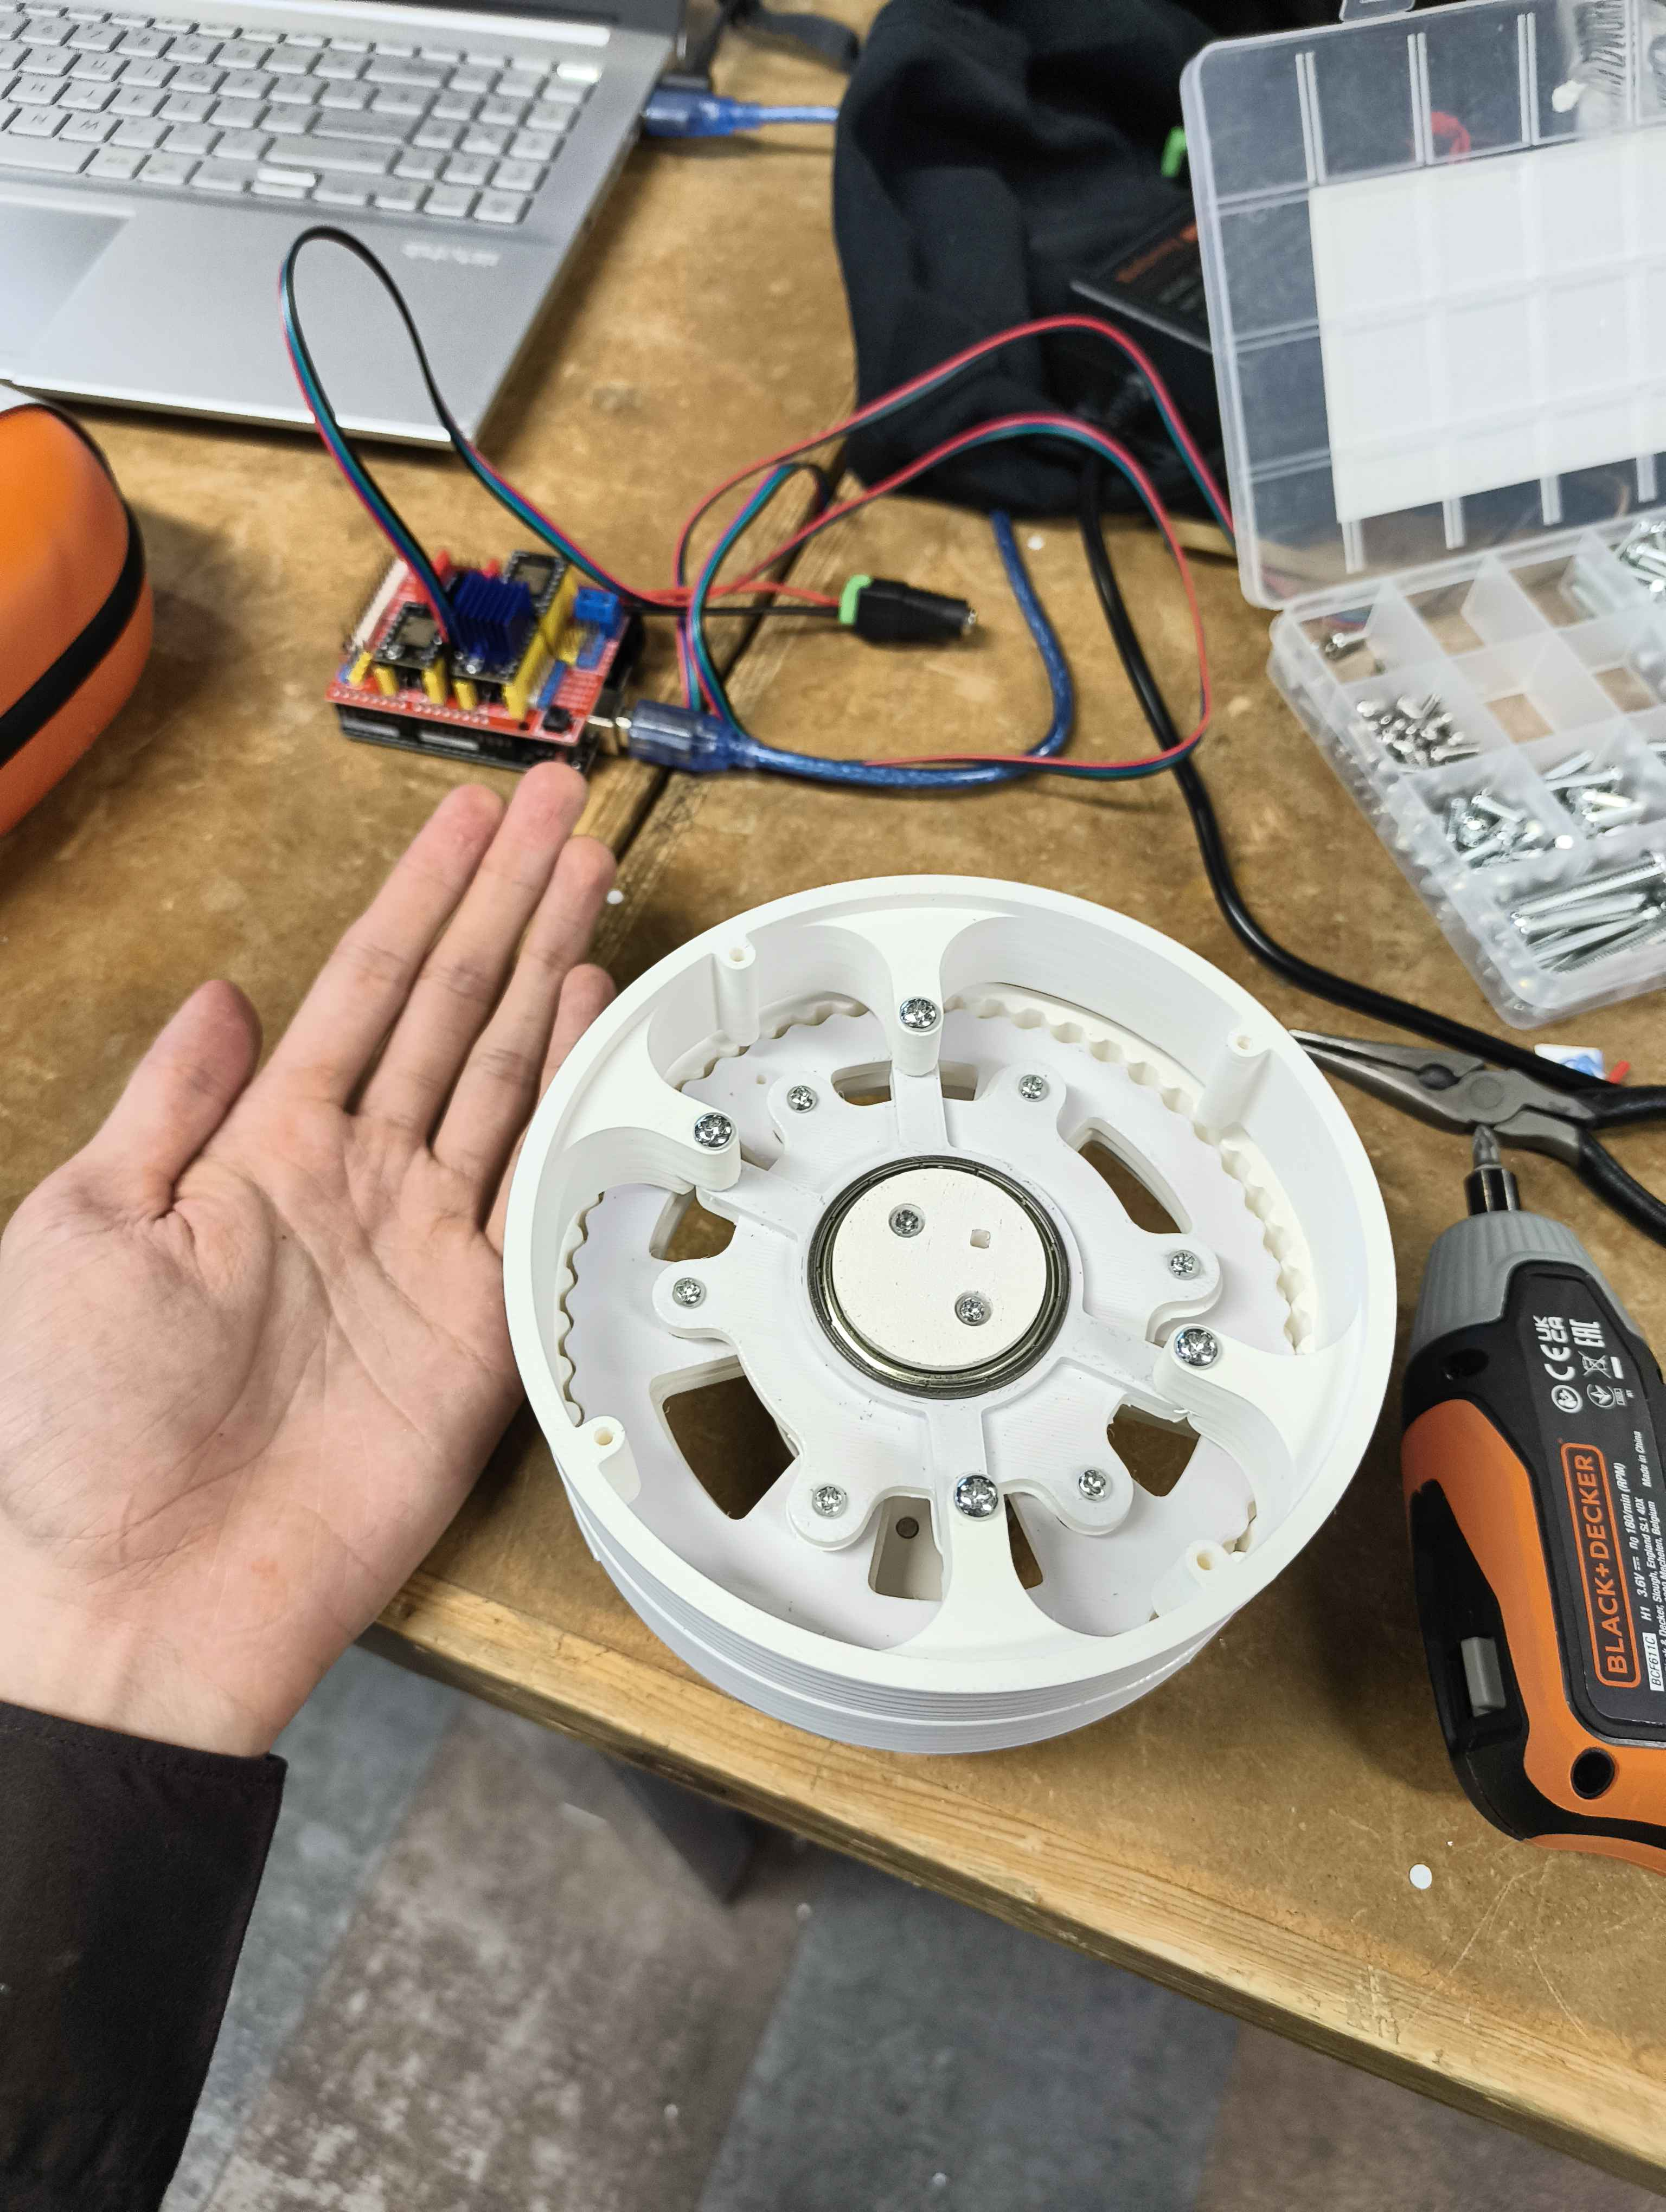
\includegraphics[width=0.6\linewidth]{img/proto2_a.jpg} 
    \caption{A photo of the second constructed prototype gearhead, author's hand for scale.}
    \label{fig:proto2}
\end{figure}

The primary cause of the low efficiency seen with the first prototype in \S~\ref{sec:proto1} was believed to be excess friction caused by poor tolerances and printed part surface finishes. The second prototype, shown in Figure \ref{fig:proto2} was thusly produced using a higher quality printer in order to improve these tolerances and surface finishes. Due to added material availability, it was also decided to scale the prototype up to the full 48:1 design. The design of this second prototype was fundamentally the same as the first, only scaled up.

Despite the improved print quality, effiency actually decreased from the initial prototype. The highest output torque achieved was roughly $1.4\,\si{N m}$, which gives an efficiency of 15\%.

\subsection{Third Prototype - 48:1 with Steel Dowels}



% --- BODY -----------------------------------------------------------------------------------------
\newpage
\section{Body, Head, \& Sensors}\label{sec:body}


% --- DEVELOPMENT ----------------------------------------------------------------------------------
\newpage
\section{Points for Development \& Timeline}\label{sec:development}

% --- BILBIOGRAPHY ---------------------------------------------------------------------------------
\newpage
\printbibliography

\end{document}